 
\begin{center}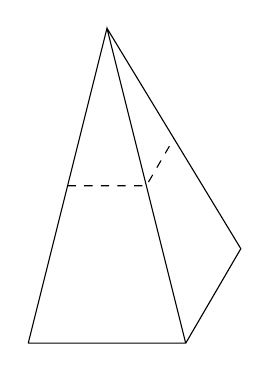
\begin{tikzpicture}
\draw(0,0)--(2,0)--(1,4)--(0,0)(2,0)--(2.7,1.2)--(1,4);
\draw[dashed](0.5,2)--(1.5,2)--(1.85,2.6);
\end{tikzpicture}\hspace{5mm}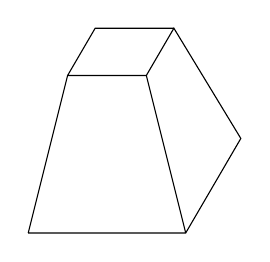
\begin{tikzpicture}
\draw(0,0)--(2,0)--(2.7,1.2)--(1.85,2.6)--(1.5,2)--(0.5,2)--(0,0) (2,0)--(1.5,2)
(0.5,2)--(0.85,2.6)--(1.85,2.6);
\end{tikzpicture}\end{center}
A frustum is formed by cutting a smaller right square pyramid from a larger right square pyramid as shown above (although the diagram is not to scale).  The height of the frustum is the half of the height of the square pyramid that was removed.  If the frustrum rests with the larger base down, as shown, its weight generates a pressure on the ground of $72$ pounds per square inch.  What pressure, in pounds per square inch, would the frustrum's weight create if the frustrum were turned upside down?\\\\


\ifsat
	\begin{enumerate}[label=\Alph*)]
	\end{enumerate}
\else
\fi

\ifacteven
	\begin{enumerate}[label=\textbf{\Alph*.},itemsep=\fill,align=left]
		\setcounter{enumii}{5}
		\item None of these. 
	\end{enumerate}
\else
\fi

\ifactodd
	\begin{enumerate}[label=\textbf{\Alph*.},itemsep=\fill,align=left]
		\item None of these. 
	\end{enumerate}
\else
\fi

\ifgridin
$162$
\else
\fi

